\documentclass{article}

% Required packages
\usepackage{amssymb}
\usepackage{amsmath}
\usepackage{graphicx}
\usepackage{geometry}
\usepackage{tikz}
\usepackage{array}
\usepackage{booktabs}
\usepackage{enumitem}
\usepackage{listings}
\usepackage{xcolor}
\usepackage{fancyhdr}
\usepackage{float}
\usepackage{subcaption}
\usepackage{comment}

% Set page geometry
\geometry{a4paper, margin=1in}

% Configure listings for Python
\lstset{
  language=Python,
  basicstyle=\ttfamily\footnotesize,
  numbers=left,
  numberstyle=\tiny\color{gray},
  frame=single,
  breaklines=true,
  breakatwhitespace=true,
  captionpos=b,
  tabsize=4,
  showspaces=false,
  showstringspaces=false,
  showtabs=false,
  commentstyle=\color{gray}\textit,
  keywordstyle=\color{blue}\bfseries,
  stringstyle=\color{red}
}

\begin{document}

\pagestyle{fancy}
\chead{DSC 257: Unsupervised Learning (Fall 2025)}
\lhead{Homework 11}
\rhead{Randall Rogers}

%------------------
% Solution for 1(a) and 1(b)
%------------------
\subsection*{Solution 1}
\noindent\rule{\textwidth}{0.4pt}\\

\subsubsection*{Solution 1 (a)}
\subsubsection*{Step 1: Identify characteristics of the dataspace}
\parbox{\textwidth}{
We are given 10 dimensional vectors where each element can be any real number ($x_{i} \in \mathbb{R}$):
}


\subsubsection*{\normalfont}{$\therefore$ we can express the dataspace $\chi$ as: $\chi = \mathbb{R}^{10}$}

\noindent\rule{\textwidth}{0.4pt}\\

\subsubsection*{Solution 1 (b)}
\subsubsection*{Step 1: Identify characteristics of the dataspace}
\parbox{\textwidth}{
We are given 3 dimensional vectors where each element is zero or one ($x_{i} \in [0,1]$):
}

\subsubsection*{\normalfont}{$\therefore$ we can express the dataspace $\chi$ as: $\chi = {[0,1]}^{3}$}

\noindent\rule{\textwidth}{0.4pt}\\

\newpage

%------------------
% Solution for 2(a),2(b), and 2(c)
%------------------
\subsection*{Solution 2}
\noindent\rule{\textwidth}{0.4pt}\\
\subsubsection*{Solution 2 (a)}
\subsubsection*{Step 1: Define Euclidean distance ($\ell_2$)}
\parbox{\textwidth}{

$$\ell_2 = \|p - q\|_2 = \sqrt{\sum_{i=1}^{n} (p_i - q_i)^2}$$

}

\subsubsection*{Step 2: Compute $\ell_2$}
\parbox{\textwidth}{
Let $p=1$ and $q=10$
$$
\begin{aligned}
\ell_2 &= \sqrt{\sum_{i=1}^{n} (p_i - q_i)^2}\\
\ell_2 &= \sqrt{\sum_{i=1}^{1} (1 - 10)^2}\\
\ell_2 &= \sqrt{(- 9)^2}\\
\ell_2 &= 9
\end{aligned}
$$
}
\subsubsection*{\normalfont}{$\therefore$ $\ell_{2} = 9$}

\noindent\rule{\textwidth}{0.4pt}\\

\subsubsection*{Solution 2 (b)}
\subsubsection*{Step 1: Define Euclidean distance ($\ell_2$)}
\parbox{\textwidth}{

$$\ell_2 = \|p - q\|_2 = \sqrt{\sum_{i=1}^{n} (p_i - q_i)^2}$$

}

\subsubsection*{Step 2: Compute $\ell_2$}
\parbox{\textwidth}{
Let $p = \begin{bmatrix} -1 \\ 12 \end{bmatrix}, q = \begin{bmatrix} 6 \\ -12 \end{bmatrix}$
$$
\begin{aligned}
\ell_2 &= \sqrt{\sum_{i=1}^{n} (p_i - q_i)^2}\\
\ell_2 &= \sqrt{(p_1 - q_1)^{2}+(p_2 - q_2)^{2}}\\
\ell_2 &= \sqrt{(-1 - 6)^{2}+(12 - (-12))^{2}}\\
\ell_2 &= \sqrt{(-7)^{2}+(24)^{2}}\\
\ell_2 &= \sqrt{625}\\
\ell_2 &= 25
\end{aligned}
$$
}
\subsubsection*{\normalfont}{$\therefore$ $\ell_{2} = 25$}

\noindent\rule{\textwidth}{0.4pt}\\


\subsection*{Solution 2}
\noindent\rule{\textwidth}{0.4pt}\\
\subsubsection*{Solution 2 (c)}
\subsubsection*{Step 1: Define Euclidean distance ($\ell_2$)}
\parbox{\textwidth}{

$$\ell_2 = \|p - q\|_2 = \sqrt{\sum_{i=1}^{n} (p_i - q_i)^2}$$

}

\subsubsection*{Step 2: Compute $\ell_2$}
\parbox{\textwidth}{
Let $p = \begin{bmatrix} 1 \\ 5 \\ -1 \end{bmatrix}, q = \begin{bmatrix} 5 \\ 2 \\ 11 \end{bmatrix}$
$$
\begin{aligned}
\ell_2 &= \sqrt{\sum_{i=1}^{n} (p_i - q_i)^2}\\
\ell_2 &= \sqrt{(p_1 - q_1)^{2}+(p_2 - q_2)^{2}+(p_3 - q_3)^{2}}\\
\ell_2 &= \sqrt{(1 - 5)^{2}+(5 - 2)^{2}+(-1 - 11)^{2}}\\
\ell_2 &= \sqrt{(-4)^{2}+(3)^{2}+(-12)^{2}}\\
\ell_2 &= \sqrt{169}\\
\ell_2 &= 13
\end{aligned}
$$
}
\subsubsection*{\normalfont}{$\therefore$ $\ell_{2} = 13$}

\noindent\rule{\textwidth}{0.4pt}\\

\newpage

%------------------
% Solution for 3(a) and 3(b)
%------------------
\subsection*{Solution 3}
\noindent\rule{\textwidth}{0.4pt}\\
\subsection*{Solution 3 (a)}
\noindent\rule{\textwidth}{0.4pt}\\
\subsubsection*{Step 1: Normalize the vector $x$}
\parbox{\textwidth}{
Let $x = \begin{bmatrix} 10 \\ 15 \\ 25 \end{bmatrix}$

$$\sum_{i=1}^{3} x_{i} = x_{1} + x_{2} + x_{3} = 10 + 15 + 25 = 50$$

Now, divide each entry by the total sum:\\

$$p = \frac{1}{50} \cdot x = \frac{1}{50} \begin{bmatrix} 10 \\ 15 \\ 25 \end{bmatrix} = \begin{bmatrix} 10/50 \\ 15/50 \\ 25/50 \end{bmatrix} = \begin{bmatrix} 0.2 \\ 0.3 \\ 0.5 \end{bmatrix}$$
}
\subsubsection*{\normalfont}{$\therefore$ the result ($p$) of scaling vertor $x$ is the following:}
$$p = \begin{bmatrix} 0.2 \\ 0.3 \\ 0.5 \end{bmatrix}$$ \\

\subsection*{Solution 3 (b)}
\noindent\rule{\textwidth}{0.4pt}\\
\subsubsection*{Step 1: Define dimension of the probability simplex}
\parbox{\textwidth}{
The dimension of vector $p$ is $3$ and $k=n-1$ where $k$ is the dimension of the probability simplex
}
\subsubsection*{\normalfont}{$\therefore$ vector $p$ lies in the probability simplex($\Delta_2$) for $k=2$}

\noindent\rule{\textwidth}{0.4pt}\\

\newpage

%------------------
% Solution for 4
%------------------
\subsection*{Solution 4}
\noindent\rule{\textwidth}{0.4pt}\\

\subsubsection*{Step 1: Understand what scaling means and the constraints of $\Delta_2$}
\parbox{\textwidth}{
Scaling a vector means multiplying all entries by the same positive constant $c > 0$.

The probability simplex $\Delta_2$ is defined as:
$$\Delta_2 = \left\{x \in \mathbb{R}^3 : x_i \geq 0 \text{ for all } i = 1,2,3, \text{ and } \sum_{i=1}^{3} x_i = 1\right\}$$

For a point to be scalable to $\Delta_2$, after scaling it must satisfy:
\begin{itemize}
\item All components must be non-negative
\item The sum of components must equal 1
\end{itemize}
}

\subsubsection*{Step 2: Find a point that violates the constraints}
\parbox{\textwidth}{
Since we need a 2-dimensional point, let's consider $x = \begin{bmatrix} a \\ b \end{bmatrix}$ where we interpret this as a 3-dimensional vector $\begin{bmatrix} a \\ b \\ 0 \end{bmatrix}$.

For any point with a negative component, scaling cannot make it non-negative. 

Example: Let $x = \begin{bmatrix} 1 \\ -2 \end{bmatrix}$

If we scale by any $c > 0$: $cx = \begin{bmatrix} c \\ -2c \end{bmatrix}$

The second component $-2c < 0$ for any $c > 0$, so this scaled vector cannot satisfy the non-negativity constraint of $\Delta_2$.
}

\subsubsection*{\normalfont}{$\therefore$ Final Answer}
Example: $x = \begin{bmatrix} 1 \\ -2 \end{bmatrix}$ (or any 2D point with at least one negative component)

\subsubsection*{\normalfont}{Graduate Level Explanation}
The key insight is that scaling preserves the sign of each component - it cannot transform negative values to positive ones. Since the probability simplex requires all components to be non-negative, any vector containing negative components cannot be scaled to lie within it. This geometric constraint is fundamental in applications like topic modeling or mixture models, where negative probabilities are meaningless. The orthant restriction (non-negativity) combined with the sum constraint defines the simplex as a bounded convex polytope, and scaling operations represent rays from the origin that either intersect this polytope or miss it entirely.

\subsubsection*{\normalfont}{Explanation for 5 year old}
Imagine you have a recipe with ingredients, but one of the "amounts" is negative - like "negative 2 cups of flour." No matter how much you shrink or grow the recipe (scaling), you'll still need a negative amount of flour, which doesn't make sense! The probability simplex is like a rule that says "all ingredients must be positive amounts," so any recipe with negative ingredients can never follow this rule, no matter how you scale it.

\noindent\rule{\textwidth}{0.4pt}\\

\newpage

%------------------
% Solution for 5
%------------------
\subsection*{Solution 5}
\noindent\rule{\textwidth}{0.4pt}\\

\subsubsection*{Step 1: Define $\Delta_3$ and identify key properties}
\parbox{\textwidth}{
The probability simplex $\Delta_3$ is defined as:
$$\Delta_3 = \left\{x \in \mathbb{R}^4 : x_i \geq 0 \text{ for all } i = 1,2,3,4, \text{ and } \sum_{i=1}^{4} x_i = 1\right\}$$

This is a 3-dimensional simplex (tetrahedron) embedded in 4-dimensional space. However, due to the constraint $\sum x_i = 1$, we can visualize it in 3D by using three coordinates and letting the fourth be determined by the constraint.

The given points are the vertices of the simplex:
\begin{itemize}
\item $\begin{bmatrix} 1 \\ 0 \\ 0 \end{bmatrix}$ corresponds to $\begin{bmatrix} 1 \\ 0 \\ 0 \\ 0 \end{bmatrix}$ in 4D
\item $\begin{bmatrix} 0 \\ 1 \\ 0 \end{bmatrix}$ corresponds to $\begin{bmatrix} 0 \\ 1 \\ 0 \\ 0 \end{bmatrix}$ in 4D
\item $\begin{bmatrix} 0 \\ 0 \\ 1 \end{bmatrix}$ corresponds to $\begin{bmatrix} 0 \\ 0 \\ 1 \\ 0 \end{bmatrix}$ in 4D
\end{itemize}
}

\subsubsection*{Step 2: Determine coordinates and sketch description}
\parbox{\textwidth}{
The fourth vertex (not shown) would be $\begin{bmatrix} 0 \\ 0 \\ 0 \\ 1 \end{bmatrix}$, which corresponds to $\begin{bmatrix} 0 \\ 0 \\ 0 \end{bmatrix}$ in our 3D representation (since the fourth coordinate is $1 - 0 - 0 - 0 = 1$).

The most central point (centroid) of the simplex is:
$$\text{centroid} = \frac{1}{4}\left(\begin{bmatrix} 1 \\ 0 \\ 0 \\ 0 \end{bmatrix} + \begin{bmatrix} 0 \\ 1 \\ 0 \\ 0 \end{bmatrix} + \begin{bmatrix} 0 \\ 0 \\ 1 \\ 0 \end{bmatrix} + \begin{bmatrix} 0 \\ 0 \\ 0 \\ 1 \end{bmatrix}\right) = \begin{bmatrix} 1/4 \\ 1/4 \\ 1/4 \\ 1/4 \end{bmatrix}$$

In 3D coordinates, this is $\begin{bmatrix} 1/4 \\ 1/4 \\ 1/4 \end{bmatrix}$.

\textbf{Sketch Description:}
\begin{itemize}
\item Draw 3D coordinate axes labeled $x_1$, $x_2$, $x_3$
\item The simplex is a triangular region (actually a tetrahedron) with vertices at:
  \begin{itemize}
  \item $(1, 0, 0)$ on the $x_1$-axis
  \item $(0, 1, 0)$ on the $x_2$-axis  
  \item $(0, 0, 1)$ on the $x_3$-axis
  \item $(0, 0, 0)$ at the origin (representing the fourth vertex)
  \end{itemize}
\item Connect these four points to form a tetrahedron
\item Mark the centroid at $(1/4, 1/4, 1/4)$
\end{itemize}
}

\subsubsection*{\normalfont}{$\therefore$ Final Answer}
The most central point in $\Delta_3$ has coordinates: $\begin{bmatrix} 1/4 \\ 1/4 \\ 1/4 \end{bmatrix}$ (or $\begin{bmatrix} 0.25 \\ 0.25 \\ 0.25 \end{bmatrix}$)

Note: The fourth coordinate is $1 - 1/4 - 1/4 - 1/4 = 1/4$

\subsubsection*{\normalfont}{Graduate Level Explanation}
The 3-simplex $\Delta_3$ is a regular tetrahedron when embedded properly in 3D space. Each vertex represents a pure probability distribution (all probability mass on one outcome), while interior points represent mixed distributions. The centroid represents the uniform distribution over 4 outcomes. This geometric structure is fundamental in Bayesian statistics, where it represents the space of all possible probability distributions over 4 categories. The simplex's convex hull property ensures that convex combinations of probability distributions remain valid probability distributions, making it a natural space for optimization in machine learning algorithms like EM or variational inference.

\subsubsection*{\normalfont}{Explanation for 5 year old}
Imagine a pyramid made of triangles (like the ones in Egypt, but pointier)! Each corner of the pyramid represents putting all your marbles in one basket - like having 100\% chocolate ice cream, or 100\% vanilla, or 100\% strawberry, or 100\% mint. The very center of the pyramid is where you have equal amounts of all four flavors - 25\% of each! Any point inside the pyramid represents some mix of the four flavors that adds up to 100\%.
\begin{figure}[h]
\centering
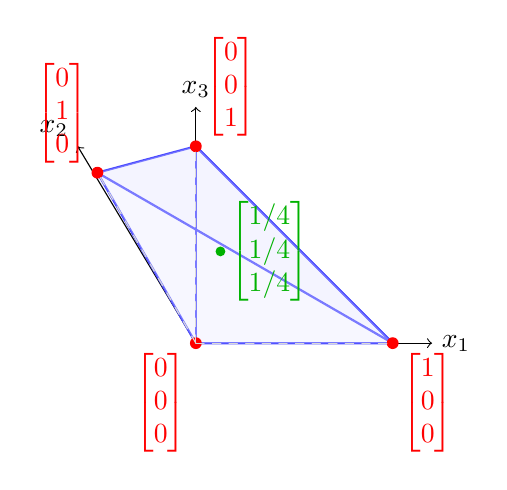
\begin{tikzpicture}[scale=2.5, line join=round, line cap=round]
% 3D coordinate system
\draw[->] (0,0) -- (1.2,0) node[right] {$x_1$};
\draw[->] (0,0) -- (-0.6,1.0) node[above left] {$x_2$};
\draw[->] (0,0) -- (0,1.2) node[above] {$x_3$};

% Tetrahedron edges (visible faces)
\draw[thick, blue!70] (1,0) -- (0,0) -- (-0.5,0.866) -- cycle;
\draw[thick, blue!70] (1,0) -- (0,1) -- (-0.5,0.866);
\draw[thick, blue!70] (0,0) -- (0,1);
\draw[thick, blue!70] (1,0) -- (0,1);

% Fill the visible triangular faces with light color
\fill[blue!10, opacity=0.3] (1,0) -- (0,0) -- (-0.5,0.866) -- cycle;
\fill[blue!15, opacity=0.3] (1,0) -- (0,1) -- (-0.5,0.866) -- cycle;

% Mark the vertices
\fill[red] (1,0) circle (0.03) node[below right] {$\begin{bmatrix} 1 \\ 0 \\ 0 \end{bmatrix}$};
\fill[red] (-0.5,0.866) circle (0.03) node[above left] {$\begin{bmatrix} 0 \\ 1 \\ 0 \end{bmatrix}$};
\fill[red] (0,1) circle (0.03) node[above right] {$\begin{bmatrix} 0 \\ 0 \\ 1 \end{bmatrix}$};
\fill[red] (0,0) circle (0.03) node[below left] {$\begin{bmatrix} 0 \\ 0 \\ 0 \end{bmatrix}$};

% Mark the centroid
\fill[green!70!black] (0.125,0.466) circle (0.025) node[right] {$\begin{bmatrix} 1/4 \\ 1/4 \\ 1/4 \end{bmatrix}$};

% Add some grid lines for reference
\draw[gray!30, dashed] (0,0) -- (1,0);
\draw[gray!30, dashed] (0,0) -- (-0.5,0.866);
\draw[gray!30, dashed] (0,0) -- (0,1);

\end{tikzpicture}
\caption{The probability simplex $\Delta_3$ showing vertices and centroid}
\end{figure}

\noindent\rule{\textwidth}{0.4pt}\\
\newpage

%------------------
% Solution for 6
%------------------
\subsection*{Solution 6}
\noindent\rule{\textwidth}{0.4pt}\\

\subsubsection*{Step 1: Recall the formulas for $\ell_1$ distance and KL divergence}
\parbox{\textwidth}{
    IDK.. LOG IS BASE e NOT 2
The $\ell_1$ distance (Manhattan distance) between two vectors $u$ and $v$ is:
$$\|u - v\|_1 = \sum_{i=1}^{n} |u_i - v_i|$$

The KL divergence between two probability distributions $P$ and $Q$ is:
$$KL(P \| Q) = \sum_{i=1}^{n} P_i \log\left(\frac{P_i}{Q_i}\right)$$
where we use the convention that $0 \log(0/Q_i) = 0$ and $P_i \log(P_i/0) = \infty$ if $P_i > 0$.
}

\subsubsection*{Step 2: Calculate each distance and divergence}
\parbox{\textwidth}{
\textbf{Part (i):} $\|p - q\|_1$ where $p = \begin{bmatrix} 1/2 \\ 1/4 \\ 1/8 \\ 1/8 \end{bmatrix}$ and $q = \begin{bmatrix} 1/4 \\ 1/4 \\ 1/4 \\ 1/4 \end{bmatrix}$

$$p - q = \begin{bmatrix} 1/2 - 1/4 \\ 1/4 - 1/4 \\ 1/8 - 1/4 \\ 1/8 - 1/4 \end{bmatrix} = \begin{bmatrix} 1/4 \\ 0 \\ -1/8 \\ -1/8 \end{bmatrix}$$

$$\|p - q\|_1 = |1/4| + |0| + |-1/8| + |-1/8| = 1/4 + 0 + 1/8 + 1/8 = 1/4 + 1/4 = 1/2$$

\textbf{Part (ii):} $\|q - r\|_1$ where $q = \begin{bmatrix} 1/4 \\ 1/4 \\ 1/4 \\ 1/4 \end{bmatrix}$ and $r = \begin{bmatrix} 1/2 \\ 0 \\ 1/4 \\ 1/4 \end{bmatrix}$

$$q - r = \begin{bmatrix} 1/4 - 1/2 \\ 1/4 - 0 \\ 1/4 - 1/4 \\ 1/4 - 1/4 \end{bmatrix} = \begin{bmatrix} -1/4 \\ 1/4 \\ 0 \\ 0 \end{bmatrix}$$

$$\|q - r\|_1 = |-1/4| + |1/4| + |0| + |0| = 1/4 + 1/4 + 0 + 0 = 1/2$$

\textbf{Part (iii):} $KL(p \| q)$

$$KL(p \| q) = \sum_{i=1}^{4} p_i \log\left(\frac{p_i}{q_i}\right)$$
$$= \frac{1}{2}\log\left(\frac{1/2}{1/4}\right) + \frac{1}{4}\log\left(\frac{1/4}{1/4}\right) + \frac{1}{8}\log\left(\frac{1/8}{1/4}\right) + \frac{1}{8}\log\left(\frac{1/8}{1/4}\right)$$
$$= \frac{1}{2}\log(2) + \frac{1}{4}\log(1) + \frac{1}{8}\log(1/2) + \frac{1}{8}\log(1/2)$$
$$= \frac{1}{2}\log(2) + 0 + \frac{1}{8}(-\log(2)) + \frac{1}{8}(-\log(2))$$
$$= \frac{1}{2}\log(2) - \frac{1}{4}\log(2) = \frac{1}{4}\log(2)$$

\textbf{Part (iv):} $KL(q \| r)$

$$KL(q \| r) = \sum_{i=1}^{4} q_i \log\left(\frac{q_i}{r_i}\right)$$
$$= \frac{1}{4}\log\left(\frac{1/4}{1/2}\right) + \frac{1}{4}\log\left(\frac{1/4}{0}\right) + \frac{1}{4}\log\left(\frac{1/4}{1/4}\right) + \frac{1}{4}\log\left(\frac{1/4}{1/4}\right)$$

Since $r_2 = 0$ and $q_2 = 1/4 > 0$, we have $\log(q_2/r_2) = \log(1/4/0) = +\infty$.

Therefore: $KL(q \| r) = +\infty$
}

\subsubsection*{\normalfont}{$\therefore$ Final Answers}
\begin{enumerate}
\item $\|p - q\|_1 = \frac{1}{2}$
\item $\|q - r\|_1 = \frac{1}{2}$
\item $KL(p \| q) = \frac{1}{4}\log(2) \approx 0.173$
\item $KL(q \| r) = +\infty$
\end{enumerate}

\subsubsection*{\normalfont}{Graduate Level Explanation}
The $\ell_1$ distance is symmetric and satisfies the triangle inequality, making it a proper metric on the probability simplex. Interestingly, both pairs have the same $\ell_1$ distance despite having different structures. The KL divergence, however, is asymmetric and not a true metric. $KL(p \| q)$ is finite because $q$ has full support (no zero entries), but $KL(q \| r) = \infty$ because $r$ has a zero entry where $q$ has positive probability. This illustrates a fundamental property: KL divergence from a distribution with full support to one with restricted support is infinite, making it useful for detecting when probability mass is assigned to impossible events in the reference distribution.

\subsubsection*{\normalfont}{Explanation for 5 year old}
The $\ell_1$ distance is like counting how much you need to move marbles between jars to make them the same - it's always the same no matter which direction you go. But KL divergence is like asking "how surprised would I be?" If one jar is completely empty but you expected marbles there, you'd be infinitely surprised! That's why one answer is infinity - it's like expecting something that's impossible.

\noindent\rule{\textwidth}{0.4pt}\\

\newpage
%------------------
% Solution for 7
%------------------
\subsection*{Solution 7}
\noindent\rule{\textwidth}{0.4pt}\\
\subsubsection*{Part a:  What is the dimensionality of each of the representations (raw pixel, HoG, VGG-last-fc, VGG-last-conv)?}
\subsubsection*{Part b:  Report test accuracies for 1-nearest neighbor classification using the various representations (raw pixel, HoG, VGG-last-fc, VGG-last-conv, random-VGG-last-fc, random-VGG-last-conv).}
\subsubsection*{Part c:  show first 5 correct/incorrect test and coresponding training for each model(raw,hog,etc.)}
% raw_acc: 35.4%
% hog_acc: 36.6%
% pretrain_cnn_acc(last_conv): 92.0%
% pretrain_cnn_acc(last_fc): 92.1%
% random_cnn_acc(last_conv): 40.6%
% random_cnn_acc(last_fc): 39.1%
\end{document}